% This is "sig-alternate.tex" V2.1 April 2013
% This file should be compiled with V2.5 of "sig-alternate.cls" May 2012
%
% This example file demonstrates the use of the 'sig-alternate.cls'
% V2.5 LaTeX2e document class file. It is for those submitting
% articles to ACM Conference Proceedings WHO DO NOT WISH TO
% STRICTLY ADHERE TO THE SIGS (PUBS-BOARD-ENDORSED) STYLE.
% The 'sig-alternate.cls' file will produce a similar-looking,
% albeit, 'tighter' paper resulting in, invariably, fewer pages.
%
% ----------------------------------------------------------------------------------------------------------------
% This .tex file (and associated .cls V2.5) produces:
%       1) The Permission Statement
%       2) The Conference (location) Info information
%       3) The Copyright Line with ACM data
%       4) NO page numbers
%
% as against the acm_proc_article-sp.cls file which
% DOES NOT produce 1) thru' 3) above.
%
% Using 'sig-alternate.cls' you have control, however, from within
% the source .tex file, over both the CopyrightYear
% (defaulted to 200X) and the ACM Copyright Data
% (defaulted to X-XXXXX-XX-X/XX/XX).
% e.g.
% \CopyrightYear{2007} will cause 2007 to appear in the copyright line.
% \crdata{0-12345-67-8/90/12} will cause 0-12345-67-8/90/12 to appear in the copyright line.
%
% ---------------------------------------------------------------------------------------------------------------
% This .tex source is an example which *does* use
% the .bib file (from which the .bbl file % is produced).
% REMEMBER HOWEVER: After having produced the .bbl file,
% and prior to final submission, you *NEED* to 'insert'
% your .bbl file into your source .tex file so as to provide
% ONE 'self-contained' source file.
%
% ================= IF YOU HAVE QUESTIONS =======================
% Questions regarding the SIGS styles, SIGS policies and
% procedures, Conferences etc. should be sent to
% Adrienne Griscti (griscti@acm.org)
%
% Technical questions _only_ to
% Gerald Murray (murray@hq.acm.org)
% ===============================================================
%
% For tracking purposes - this is V2.0 - May 2012

\documentclass{sig-alternate-05-2015}
\usepackage{hyperref}

\begin{document}

% Copyright
%\setcopyright{acmcopyright}
%\setcopyright{acmlicensed}
%\setcopyright{rightsretained}
%\setcopyright{usgov}
%\setcopyright{usgovmixed}
%\setcopyright{cagov}
%\setcopyright{cagovmixed}
\title{Home Depot Product Search Relevance}
\subtitle{[Kaggle Competition]
\titlenote{This competition can be found at this site:\\
\texttt{https://www.kaggle.com/c/home-depot-product-search-relevance}}}
%
% You need the command \numberofauthors to handle the 'placement
% and alignment' of the authors beneath the title.
%
% For aesthetic reasons, we recommend 'three authors at a time'
% i.e. three 'name/affiliation blocks' be placed beneath the title.
%
% NOTE: You are NOT restricted in how many 'rows' of
% "name/affiliations" may appear. We just ask that you restrict
% the number of 'columns' to three.
%
% Because of the available 'opening page real-estate'
% we ask you to refrain from putting more than six authors
% (two rows with three columns) beneath the article title.
% More than six makes the first-page appear very cluttered indeed.
%
% Use the \alignauthor commands to handle the names
% and affiliations for an 'aesthetic maximum' of six authors.
% Add names, affiliations, addresses for
% the seventh etc. author(s) as the argument for the
% \additionalauthors command.
% These 'additional authors' will be output/set for you
% without further effort on your part as the last section in
% the body of your article BEFORE References or any Appendices.

\numberofauthors{3} %  in this sample file, there are a *total*
% of EIGHT authors. SIX appear on the 'first-page' (for formatting
% reasons) and the remaining two appear in the \additionalauthors section.
%
\author{
% You can go ahead and credit any number of authors here,
% e.g. one 'row of three' or two rows (consisting of one row of three
% and a second row of one, two or three).
%
% The command \alignauthor (no curly braces needed) should
% precede each author name, affiliation/snail-mail address and
% e-mail address. Additionally, tag each line of
% affiliation/address with \affaddr, and tag the
% e-mail address with \email.
%
% 1st. author
\alignauthor
Hao Mao\\
%\titlenote{}\\
       \affaddr{Northeastern University}\\
       \affaddr{Seattle, WA}\\
       \email{mao.ha@husky.neu.edu}
% 2nd. author
\alignauthor
Wanting Jiang\\
%\titlenote{}\\
       \affaddr{Northeastern University}\\
       \affaddr{Seattle, WA}\\
       \email{jiang.wa@husky.neu.edu}
% 3rd. author
\alignauthor Mingzhe Xu\\
%\titlenote{}\\
       \affaddr{Northeastern University}\\
       \affaddr{Seattle, WA}\\
       \email{xu.ming@husky.neu.edu}
\and  % use '\and' if you need 'another row' of author names
}

\maketitle
\begin{abstract}

Search relevancy is an implicit measure Home Depot uses to gauge how quickly they can get customers to the right products. Currently, human raters evaluate the impact of potential changes to their search algorithms, which is a slow and subjective process. By removing or minimizing human input in search relevance evaluation, Home Depot hopes to increase the number of iterations their team can perform on the current search algorithms. In this paper, we first use stemming and other approached to do feature engineering. Then, after comparing with other models, we apply Random Forest to predict the relevancy between search queries and the products in a gauge of number 1 to 3 in an effort to make accurate and efficient prediction. We finally achieved 0.47105 which ranks 340 in the Leaderboard, with more than 2000 teams and the first one scored 0.43294.
\end{abstract}

%
% End generated code
%

%
%  Use this command to print the description
%
\printccsdesc

% We no longer use \terms command
%\terms{Theory}

\keywords{Search Relevance; Nature Language Processing; Home Depot; Random Forest; Stemming}

\section{Introduction}
Shoppers rely on Home Depot's product authority to find and buy the latest products and to get timely solutions to their home improvement needs. From installing a new ceiling fan to remodeling an entire kitchen, with the click of a mouse or tap of the screen, customers expect the correct results to their queries quickly. Speed, accuracy and delivering a frictionless customer experience are essential.\\

Our goal is to develop a model that can improve Home Depot's customers' shopping experience and accurately predict the relevance of search results and products. Based on the data from Home Depot, we are going to predict a relevance score for the provided combinations of search terms and products. We have applied a couple of tool kits for our data processing and model application, such as SnowballStemmer, Sci-kit Learn, Pandas etc..This project contains three parts: data preprocessing, which includes cleaning, merging, stemming, feature selection and adding new attributes, application of Random Forest model, and the evaluation of  the models based upon Root Mean Squared Error. \\

This paper is structured as follow. First, the original datasets we adopted from Kaggle is described and explained, which is followed by how the data was preprocessed so as to generate features that can be used in models including stemming and generating new features. Then, there will be a discussion of choosing Random Forest over other models and how it works. Finally the preliminary empirical result will be displayed and elaborated. 

\section{Datasets}

Datasets for this project are from Home Depot's website which contains a number of products and real customer search terms. To create the ground truth labels, Home Depot has crowdsourced the search/product pairs to multiple human raters. Each pair in the dataset was evaluated by at least three human raters. The rate values are from 1 to 3, where 3 is the most relevant, 2 somewhat relevant and 1 irrelevant. The provided relevance scores are the average values of the ratings. We adopt the data from Kaggle website including mainly the training data and testing data.\\

\subsection{Datasets Description}
Here are the original datasets provided by Kaggle.com:
\begin{table}[ht]
\centering
\caption{Datasets Description}
\label{my-label}
\begin{tabular}{|l|l|}
\hline
\textbf{Dataset Name}  & \textbf{Dataset Description}  \\ \hline
train.csv 		   	  & the training set, contains \\
			           & products, searches, and \\
			           & relevance scores \\ \hline
product\_descriptions.csv & contains a text description \\
				& of each product \\ \hline
attributes.csv      	   & provides extended information \\
 				   & about a subset of the products \\
				   & (typically representing detailed\\
				   &  technical specifications). \\
				   & Not every product will have \\
				   & attributes.\\ \hline
test.csv 	   		&  the test set, contains products \\
				& and searches. (We will provide \\
				& our prediction of the relevance \\
				& of those pairs)\\ \hline
\end{tabular}
\end{table}

We merge the train.csv file and product\_descriptions.csv file as our new training data so as to get the concrete description for the product. The attributes are also merged into the training data so as to make the most of the given data. After merging all the data into one dataset, we can preprocess the data into features that are usable for modeling. \\
\subsection{Data Field Description}
\begin{table}[ht]
\centering
\caption{Data Field Description}
\label{my-label}
\begin{tabular}{|l|l|}
\hline
\textbf{Field Name}  & \textbf{Field Description}  \\ \hline
id 				   & a unique Id field which represents \\
			            & a (search\_term, product\_uid) pair \\ \hline
product\_uid                 & an id for the products \\ \hline
product\_title       	   & name of the product   \\ \hline
product\_description 	   & the text description of the \\
				   & product (may contain HTML \\ 
				   & content)         \\ \hline
search\_term		   & the search query in text form \\\hline
relevance			   & the average of the relevance \\
				   & ratings for a given id\\ \hline
name		 	   & name of the attribute \\ \hline
value			   & value of the attribute \\ \hline
\end{tabular}
\end{table}
The training data and product description data also provide the above data fields which can be later applied as features. However, features such as product description or search term can not be directly used and also have potential to be restructured to generate new features. So in bellow preprocessing part we will elaborate on how we manipulate the original data to generate features for our model.

\section{Algorithms}
In this project, the most crucial part is feature engineering. In our given data, there are just product title, attribute and description for product information. And on the user side, we only have query data. Therefore, cleaning data, trimming features, and generating new data is the key to a more accurate prediction in this case.

\subsection{Preprocessing}
There are two kinds of attributes in the dataset. The first one is some common attributes, which all products have that, such as title and product description. Another one is extended information which means not every product will have these attributes, such as Brand and Length.\\
\begin{table}[ht]
\centering
\caption{List of Features}
\begin{tabular}{|c|c|l|} \hline
Common Attributes & Extended Attributes \\\hline
\ Title & Brand\\
\ Production Description & Material \\
\  & Length\\ 
\   & Weight\\ 
\   & Width\\
\   & Search\_Term\\
\   & Bullets \\
\   & Bullet01\\
\   & Bullet02\\
\   & Bullet03\\
\   & Bullet04\\
\  & ... \\ \hline\end{tabular}
\end{table}

All common attributes are considered important here, we will use all of them in our predict model.\\

Some extended attributes are also very useful in calculating search relevance, such as Brand, Material and Functionality, which are as important as the Title. We will focus on these attributes.\\

Other extended attributes like Length, Bullet01, which might be helpful in our calculation. But it is hard to decide which one should be used in the model, so in our experiment, we will test several combination of the attributes, and choose the best as our final selected attributes.

\subsubsection{Data Cleaning}
The given raw data contains various forms of words and the difference in the style make is hard to give accurate prediction. Therefore, we first clean up the data with the following approaches. First, for all the capitalized or uppercase words/letters, we lowercase them so that the data is robust to the case sensitiveness. Second, we remove punctuations. Punctuation is helpful when we read, but in models it is hard to incorporate them without affecting the accuracy. Third, we digitalize all the quantities such as one oz transferred to 1oz. Fourth, units are unified into abbreviations, such as 5 inches transferred into 5in.. Fifth, we corrected mis-spelt words, such as \lq \textit{correet}' was updated to \lq \textit{correct}'. 

\subsubsection{Data Stemming}
In order to improve the precision of the result, we will use Snowball to do stemming on the selected attributes and queries.\cite{snowball} Other than applying given Snowball stemming tool to do basic stemming, we also explore the data and add more stemming methods in our preprocessing stage. There are many units shown in the data such as unit of length, unit of weight, unit of space, etc. We unified the various impressions into one. For example, ``\textit{inches}", ``\textit{in}" or ``\textit{inch}" are all stemmed into ``\textit{in}."; ``\textit{pound}", ``\textit{pounds}", ``\textit{lbs}" and ``\textit{lb}" are stemmed into ``lb.". We also eliminate punctuations and redundant space in the text.

\subsubsection{Data Normalizations}
Instead of simply assigning same weight to all the words in the attributes, we applied tf-idf to normalize data fields that are consists of words. We calculate the term frequency-inverse document frequency ratio of a word in search query or product description.\cite{tf-idf, tf-idf1} This feature is very useful in terms of the importance or the weight of a word in the text.

\subsubsection{Feature Preparation}
For the purpose of getting the importance of the word in the attributes, we calculate the ratio of each word in each attribute, based on the length of the query. In addition to the original features, we generated new features based on the original data. We generate bullets feature which combined all bullets of a product into one. We also combined search term with product title into a new feature called product info. \\

After preparing the features, we generated a final training dataset, with 23 columns in total, including id, relevance, brand, search\_term, product\_description, product\_title, and product\_info, len\_of\_title, len\_of\_description, len\_of\_brand, query\_in\_title, query\_in\_description, query\_last\_word\_in\_title, query\_last\_word\_in\_description, ratio\_title, ratio\_description, word\_in\_brand, ratio\_brand, search\_term\_feature. For some of the numeric features, we calculated the properties and here are the description of those features in our final training dataset.\\

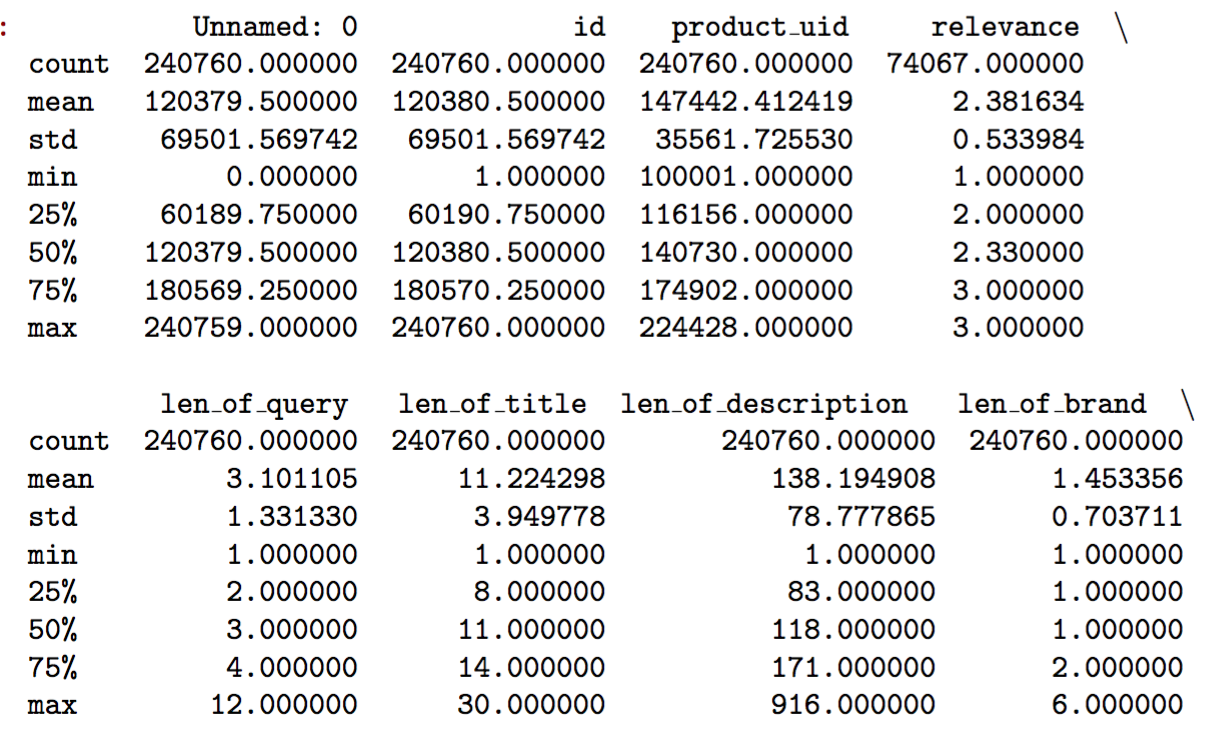
\includegraphics[width=8cm, height=5cm]{scr-id.png}\\
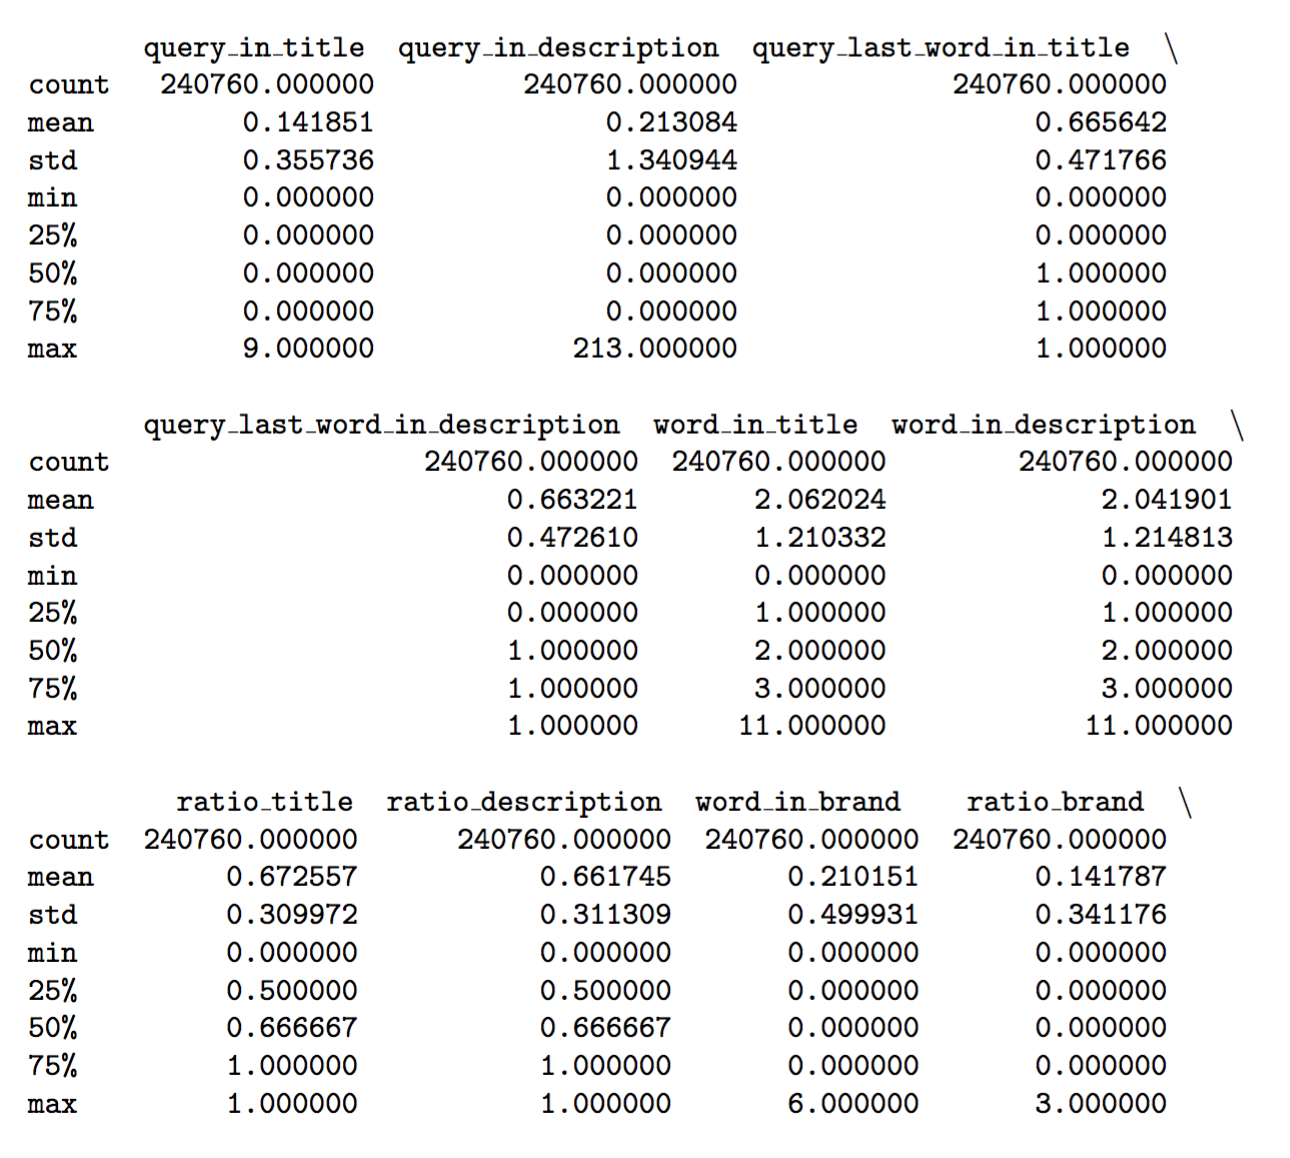
\includegraphics[width=8cm, height=8cm]{scr-query.png}

\subsection{Modelling}
With features prepared for the model, we then compare different models to apply based on their pros and cons. Random forest is better at feature selection given that we have many features to choose from.\cite{rf0} It is also very robust against overfitting.\cite{rfwiki, rf1} Naive Bayes is easy to train and understand. However, it based on the "naive" assumption that all variables are uncorrelated with each other. What's more it is fragile to overfitting compared with Random Forest. Regarding logistic regression, it is hard for it to handle features that are non-linear. What's more, Random Forest is very powerful when handling large dataset with high dimensions.\cite{rf2, rf3} Therefore we choose Random Forests as our core method.

\subsubsection{Model Selection}
There are many features in products and items and we are not sure which features play important on search result relevancy. Also this project already provides us some training results. So we can use Random Forest model with current training data to predict the relevance for each pair listed in the test set by trying different feature sets. Given the Random Forest model, it is easier for us to pick the best feature set and an accurate predicting model.

\subsubsection{Random Forest}
Random forests is a notion of the general technique of random decision  
forests that are an ensemble learning method for classification, regression and 
other tasks, that operate by constructing a multitude of decision trees at training time and outputting the class that is the mode of the classes (classification) or mean prediction (regression) of the individual trees. Random decision forests correct for decision trees' habit of overfitting to their training set.

\subsubsection{Mechanism of Random Forest}
When the training set for the current tree is drawn by sampling with replacement, about one-third of the cases are left out of the sample. This OOB (out-of-bag) data is used to get a running unbiased estimate of the classification error as trees are added to the forest. It is also used to get estimates of variable importance.\\

After each tree is built, all of the data are run down the tree, and proximities are computed for each pair of cases. If two cases occupy the same terminal node, their proximity is increased by one. At the end of the run, the proximities are normalized by dividing by the number of trees. Proximities are used in replacing missing data, locating outliers, and producing illuminating low-dimensional views of the data.

\subsubsection{Application of Random Forest Model}

First, pick a feature set that contains relevant features. Here we choose \lq id', \lq relevance', \lq search\_term', \lq product\_title', \lq product\_description', \lq product\_info',\lq attr', \lq brand', \lq bullets', \lq bullet1', \lq bullet2', \lq bullet3', \lq bullet4', \lq material'. Second, we build a Random Forest Model based on this feature set. However, we did not simply put those features into the model. Pipeline is used to transform some of our key features. For ``search\_term", ``product\_title", and ``brand", we calculate the tf-idf and truncated the tf-idf matrix into one-dimensional feature by using singular value decomposition (SVD) so as to increase the accuracy and improve the efficiency. We then union the features into the data, and prepare the features thoroughly for the model.\\

Then, we apply grid search for optimizing hyper-parameters. Instead of using randomized search, grid search is slightly slower, yet it is more accurate and has better performance than randomized search.\cite{grid} After setting up the estimator and parameters for grid search, we run fit the model with our training data and predict the parameters for our model.\\

Finally, After fitting the training data and get the best params and best score, we calculate the Root Mean Squared Error (RMSE) evaluation for this model to gauge the model. We also submitted our result to Leaderboard and got our first score on Kaggle Leaderboard which beats the benchmarks and better than hundreds other submissions. \\
\section{Evaluation Method}
The evaluation we use, or based on Kaggle's evaluating standards, RMSE is used, which is the square root of the mean/average of the square of all of the error. The use of RMSE is very common and it makes an excellent general purpose error metric for numerical predictions. \cite{kaggle} Compared to the similar Mean Absolute Error, RMSE amplifies and severely punishes large errors.\\
\begin{eqnarray*}
RMSE & = &\sqrt{ \frac{1}{n} \sum_{i = 1}^{n}({\mathbf{y}_i  -  \hat{\mathbf{y}_i})}} \\
\end{eqnarray*}
In python, RMSE = mean\_squared\_error(y, y\_pred)**0.5. Kaggle uses this number as the score reference in it's Leaderboard.

\section{Empirical Result}

We've conducted five sets of experiment with random forest with different set of features and our rank in leaderboard varies for each submission. These three experiments are called easy forest, complex forest with less features, and complex forest with more features. \\

In the first experiment, we incorporate features from original data without any modification such as cleaning or stemming. This model yields a RMSE of 0.48721. In the second experiment, we modify the features by cleaning them and processed with stemming. Based on the data we acquired after the above cleaning, stemming, and normalizing, there are 11 features selected to build a satisfying model. Those features we included are id,  product\_title, product\_uid, relevance, search\_term, product\_description, brand, product\_info, len\_of\_query, word\_in\_title, word\_in\_description. The score has improved by 0.003, which is 0.48462. However, none of these two experiments adopted data transformation, which is a deep modification of the original data.\\

In our third experiment, we generated a bunch of new features. The features we've adopted are  id,  product\_title, product\_uid, relevance, search\_term, product\_description, brand, product\_info, len\_of\_query, word\_in\_title, word\_in\_description, brand\_feature, and search\_term\_feature. In total of 13 features. Also, we used tf-idf on search\_term, product\_title and brand and generated new features for this model. In the meantime, some of the features, such as id, relevance, brand, search\_term, product\_description, product\_title, and product\_info, after being transformed or found less significant, are discarded. In this experiment, the score is 0.47939, which is higher than the previous experiment by 0.005. And our rank in Leaderboard increased accordingly.\\

Next, we tried to use more features we generated. Features such as the lengths, the last word, words of query shown in title, ratios etc are taken into the model. And we initially include 23 features, including id, relevance, brand, search\_term, product\_description, product\_title, and product\_info, len\_of\_title, len\_of\_description, len\_of\_brand, query\_in\_title, query\_in\_description, query\_last\_word\_in\_title, query\_last\_word\_in\_description, ratio\_title, ratio\_description, word\_in\_brand, ratio\_brand, search\_term\_feature. Like the previous experiment, we also dropped less significant features and calculate tf-idf for search\_term, product\_title and brand, with weight or 0.5, 0.25, 0.25 respectively. With more features added, this model is more robust than the previous one which has less features, and the RMSE is improved to 0.47181, which is 0.008 lower, with the rank increased to around 300.\\

After we have a set of features and the model is chosen, it is really difficult to improve the result even slightly after 3 or 4 rounds of improvements. But we managed to decrease the RMSE after trying many approaches.\\

Our fifth experiment is to modify the transformed feature especially tf-idf feature. The above 23 features performs good in our previous experiment so they are kept in this experiment as well. Regarding tf-idf feature, we decided to include product\_description, and redistributed the weight for each tf-idf feature. For search\_term, product\_title, product\_description and brand, we assigned 0.5, 0.25, 0.1 and 0.5 respectively. And the result of our RMSE dropped to 0.47105, which is slightly better than the previous experiment.




\begin{thebibliography}{9}
\bibitem{latexcompanion} 
Hastie, Trevor; Tibshirani, Robert; Friedman, Jerome.
\textit{The Elements of Statistical Learning}. 
Springer, 2001.

\bibitem{rf0} 
 Leo Breiman.
\textit{Random Forests}. Machine Learning,
October 2001, Volume 45, Issue 1, pp 5-32.

\bibitem{snowball} 
SnowBall:
\texttt{http://snowball.tartarus.org/}. 
 
\bibitem{rfwiki} 
Random Forest Wikipedia,
\\\texttt{https://en.wikipedia.org/wiki/Random\underline{\hspace{.2cm}}forest}

\bibitem{rf1}
Liaw, Andy, and Matthew Wiener. "Classification and regression by randomForest." R news 2.3 (2002): 18-22.

\bibitem{rf2}
Ho, Tin Kam (1995). Random Decision Forests (PDF). Proceedings of the 3rd International Conference on Document Analysis and Recognition, Montreal, QC, 14-16 August 1995. pp. 278-282

\bibitem{rf3}
Breiman, Leo (2001). "Random Forests". Machine Learning 45 (1): 5-32.

\bibitem{grid}
Scikit-Learn: Comparing randomized search and grid search for hyperparameter estimation:\\
\href{url}{http://scikit-learn.org/stable/auto\_examples/model\_selection/randomized\_search.html}

\bibitem{tf-idf1}
Ramos, Juan. "Using tf-idf to determine word relevance in document queries." Proceedings of the first instructional conference on machine learning. 2003.

\bibitem{tf-idf}
Joachims, Thorsten. A Probabilistic Analysis of the Rocchio Algorithm with TFIDF for Text Categorization. No. CMU-CS-96-118. Carnegie-mellon univ pittsburgh pa dept of computer science, 1996.
\bibitem{kaggle}
Kaggle Competition: \href{url}{https://www.kaggle.com/wiki/RootMeanSquaredError}

\end{thebibliography}

%
%\begin{figure}
%\centering
%\includegraphics{fly}
%\caption{A sample black and white graphic.}
%\end{figure}

%\begin{figure}
%\centering
%\includegraphics[height=1in, width=1in]{fly}
%\caption{A sample black and white graphic
%that has been resized with the \texttt{includegraphics} command.}
%\end{figure}

\end{document}
